\documentclass[11pt,table]{beamer}
\usepackage[utf8]{inputenc}
\usepackage[T1]{fontenc}
\usepackage{amsmath}
\usepackage{amsfonts}
\usepackage{amssymb}
\usepackage{mathtools}
\usepackage{graphicx}
\usepackage{subfigure}
\usepackage{ulem}

\setbeamertemplate{navigation symbols}{}
\usepackage{appendixnumberbeamer}

\usepackage{listings}
\usepackage{multicol}
\lstdefinelanguage
   [x64]{Assembler}     % add a "x64" dialect of Assembler
   [x86masm]{Assembler} % based on the "x86masm" dialect
   % with these extra keywords:
   {morekeywords={CDQE,CQO,CMPSQ,CMPXCHG16B,JRCXZ,LODSQ,MOVSXD, %
                  POPFQ,PUSHFQ,SCASQ,STOSQ,IRETQ,RDTSCP,SWAPGS, %
                  rax,rdx,rcx,rbx,rsi,rdi,rsp,rbp, %
                  r8,r8d,r8w,r8b,r9,r9d,r9w,r9b, %
                  r10,r10d,r10w,r10b,r11,r11d,r11w,r11b, %
                  r12,r12d,r12w,r12b,r13,r13d,r13w,r13b, %
                  r14,r14d,r14w,r14b,r15,r15d,r15w,r15b}} % etc.

\usepackage{xcolor}
\definecolor{pale-red}{HTML}{FFCCCC}
\definecolor{pale-yellow}{HTML}{EEEEBB}
\definecolor{pale-green}{HTML}{CCDDAA}


\usepackage{tikz}
\usetikzlibrary{chains}
\usetikzlibrary{shapes.geometric}
\tikzset{box/.style = {draw, rounded corners, on chain, align=center, text centered}}
\tikzset{start/.style = {draw, rounded corners, on chain, align=center, text centered, fill=pale-green}}
\tikzset{stop/.style = {draw, rounded corners, on chain, align=center, text centered, fill=pale-red}}
\tikzset{decision/.style = {draw, rounded corners, on chain, align=center, text centered, fill=pale-yellow}}
\tikzset{arr/.style = {very thick, -latex}}


\usetheme{CambridgeUS}
\begin{document}

\author{Lisa Jones}
\title{Mathematics in Cyber Security}
%\subtitle{}
%\logo{}
%\institute{}
%\date{}
%\subject{}
%\setbeamercovered{transparent}
%\setbeamertemplate{navigation symbols}{}
\frame[plain]{\maketitle}

% start by defining cyber security (note that this is opinion, colored by the flavor of research one dones)
% "no device under your control is executing code not under your control, or performing computations that yield information other than the intended result"

\begin{frame}
\frametitle{What is program analysis?}
  \begin{itemize}
  \item{ Automatically analyzing the behavior of computer programs regarding a property such as correctness, robustness, safety and liveness}
    % give informal description of safety (temporal and memory)
    \medskip
  \item{Can be \textit{static} (performed without running the program), \textit{dynamic}, or a hybrid of both}
    % note that we are talking about dynamic
      \end{itemize}
  \end{frame}

\begin{frame}
  \frametitle{Toy example}

  Let $ foo: int \times int \times List[int] \times int \to Maybe(int) $
  be a function such that
  \[
  foo(x, op, arr, n) = \begin{cases}
    \sum_{i=0}^{n} arr_i & \mbox{if } x \neq 0 \mbox{ and } op=0 \\
    \prod_{i=0}^{n} arr_i & \mbox{if } x \neq 0 \mbox{ and } op=1 \\
    undefined & \mbox{otherwise (i.e., } x=0 \mbox{ or } op \not\in \{0, 1\})
  \end{cases}
  \]
  
  \end{frame}

\begin{frame}[fragile]
  \frametitle{Toy program}
  \lstinputlisting[language=C, linerange={2-25}, basicstyle=\scriptsize]{example.c}
  \end{frame}


\begin{frame}
\frametitle{What is discrete mathematics?}
  \begin{itemize}
  \item{Study of mathematical structures (sets + features) that do not vary ``smoothly'', but have distinct, separated values}
    % what I mean by smoothly: there exists a bijection between elements of the set I'm working with and (some finite subset of) the naturals; no bijection to the reals
    \medskip
  \item{Examples: integers, graphs, statements in logic}
  \end{itemize}
\end{frame}



  \begin{frame}
\frametitle{What is a graph?}
\begin{definition} A \textbf{graph} is a pair  G = (V, E) ,
  where V is a set whose elements are called \textit{vertices} and
  E is a set whose elements are paired vertices, called \textit{edges}.
  If the elements of E are ordered pairs, we call the graph \textit{directed}; otherwise, we call it \textit{undirected}.
\end{definition}
\bigskip
\begin{definition}
  A \textbf{path} in a graph is a sequence of edges which joins a sequence of (distinct) vertices. Paths in directed graphs have an added restriction: the edges must all be directed in the same direction.
\end{definition}
  \end{frame}

  \begin{frame}
\frametitle{What is a graph?}
% Insert picture of a directed graph with a path highlighted
\begin{columns}
  \column{.48\linewidth}{
      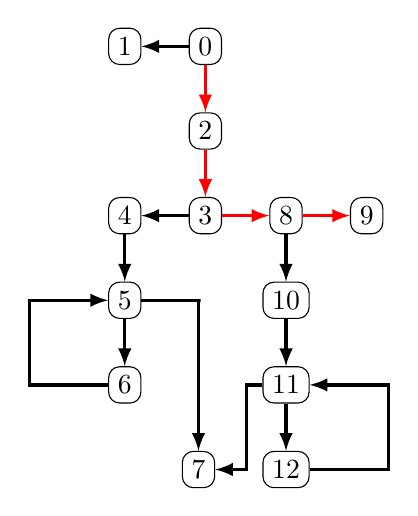
\begin{tikzpicture}[auto,
  start chain = going below,
  node distance = 6 mm,
  %% box/.style = {draw, rounded corners, on chain, align=center},
  %% arr/.style = {very thick, -latex}
]

\node[box] (b0) {0};
\node[box, left=of b0] (b1) {1};
\node[box, below=of b0] (b2) {2};
\node[box, below=of b2] (b3) {3};
\node[box, left=of b3] (b4) {4};
\node[box, below=of b4] (b5) {5};
\node[box, below=of b5] (b6) {6};
% b12 needs to be defined before b7
\node[box, right=of b3] (b8) {8};
\node[box, right=of b8] (b9) {9};
\node[box, below=of b8] (b10) {10};
\node[box, below=of b10] (b11) {11};
\node[box, below=of b11] (b12) {12};
\node[box, left=of b12] (b7) {7};

\draw[arr]  (b0) -- (b1);
\draw[arr, draw=red]  (b0) -- (b2);
\draw[arr, draw=red]  (b2) -- (b3);
\draw[arr]  (b3) -- (b4);
\draw[arr, draw=red]  (b3) -- (b8);
\draw[arr, draw=red]  (b8) -- (b9);
\draw[arr]  (b8) -- (b10);
\draw[arr]  (b10) -- (b11);
\draw[arr]  (b11) -- (b12);
\draw[arr]  (b12.east) -- ++ (1, 0) |- (b11);
\draw[arr]  (b11) -- ++ (-.5, 0) |- (b7.east);
\draw[arr]  (b4) -- (b5);
\draw[arr]  (b5) -- (b6);
\draw[arr]  (b6.west) -- ++ (-1,0) |- (b5);
\draw[arr]  (b5.east) -- ++ (.75, 0) -| (b7.north);


\end{tikzpicture}
  
    }
  \column{.52\linewidth}{
\begin{align*}
  G &= (V, E) \\[10pt]
  V &= \{0, 1, ..., 12\} \\[10pt] 
  E &= \{ (0, 1), (0, 2), (2, 3), (3, 4),\\ 
  & (3, 8), (8, 9), (8, 10), (10, 11),\\
  & (11, 12), (12, 11), (11, 7),\\
  & (4, 5), (5, 6), (6, 5), (6, 7) \}
\end{align*}

Node $9$ is \textbf{\textit{reachable}} from node $0$ by path $((0,2), (2, 3), (3, 8), (8, 9))$.
    }
\end{columns}
  \end{frame}


  \begin{frame}
\frametitle{Graphs in program analysis}
Control-flow graph:
\bigskip
\begin{itemize}
  \item{Nodes - \textit{basic blocks} of a program}
    \medskip
  \item{Edges - \textit{control flow} between basic blocks}
      \end{itemize}
  \end{frame}

  
  \begin{frame}[fragile]
    \frametitle{How we actually build control flow graphs}
    \vspace{-.75cm}\lstinputlisting[language={[x64]Assembler}, linerange={6-74}, basicstyle=\tiny\linespread{0.1}, multicols=2]{example.s}
    % highlight that this is asm for foo, compiled for x86_64, in intel syntax, with no optimization
  \end{frame}


  \begin{frame}
    \frametitle{High-level control-flow graph}
    \vspace{-.75cm}\centering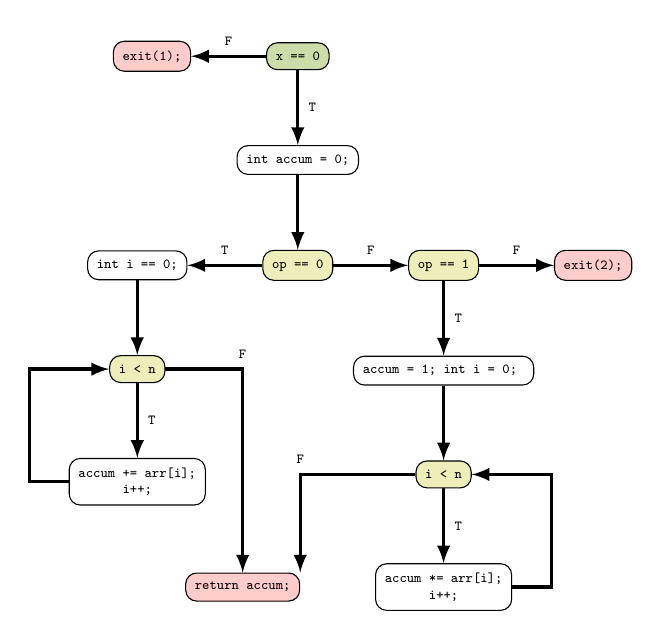
\begin{tikzpicture}[auto,
  start chain = going below,
  node distance = .95 cm,
  font=\tiny\ttfamily
]

\node[decision, fill=pale-green] (b0) {x == 0};
\node[stop, left=of b0] (b1) {exit(1);};
\node[box, below=of b0] (b2) {int accum = 0;};
\node[decision, below=of b2] (b3) {op == 0};
\node[box, left=of b3] (b4) {int i == 0;};
\node[decision, below=of b4] (b5) {i < n};
\node[box, below=of b5] (b6) {
  accum += arr[i]; \\
  i++;
};
% b12 needs to be defined before b7
\node[decision, right=of b3] (b8) {op == 1};
\node[stop, right=of b8] (b9) {exit(2);};
\node[box, below=of b8] (b10) {
  accum = 1;
  int i = 0;
};
\node[decision, below=of b10] (b11) {i < n};
\node[box, below=of b11] (b12) {
  accum *= arr[i];\\
  i++;
};
\node[stop, below=of b3, left=of b12] (b7) {return accum;};

\draw[arr]  (b0) -- (b1) node[midway, above]{F};
\draw[arr]  (b0) -- (b2) node[midway, right]{T};
\draw[arr]  (b2) -- (b3);
\draw[arr]  (b3) -- (b4) node[midway, above]{T};
\draw[arr]  (b3) -- (b8) node[midway, above]{F};
\draw[arr]  (b8) -- (b9) node[midway, above]{F};
\draw[arr]  (b8) -- (b10) node[midway, right]{T};
\draw[arr]  (b10) -- (b11);
\draw[arr]  (b11) -- (b12) node[midway, right]{T};
\draw[arr]  (b12.east) -- ++ (.5, 0) |- (b11);
\draw[arr]  (b11) -- ++ (-.75, 0) -| (b7.north east) node[midway, above]{F};
\draw[arr]  (b4) -- (b5);
\draw[arr]  (b5) -- (b6) node[midway, right]{T};
\draw[arr]  (b6.west) -- ++ (-.5,0) |- (b5);
\draw[arr]  (b5.east) -- ++ (.25, 0) -| (b7) node[midway, above]{F};



\end{tikzpicture}

  \end{frame}
  
  %% \begin{frame}
  %%   \frametitle{Example program analyses}
  %%   \begin{itemize}
  %%   \item{\textbf{Control-flow analysis}: what functions get called}
  %%     \medskip
  %%   \item{\textbf{Data-flow analysis}: what ranges of values variables take} 
  %%   \end{itemize}
  %% \end{frame}
  
  
%% \begin{frame}
%% \frametitle{Example: finding an input to reach a desired state}
%% \vspace{-.75cm}\centering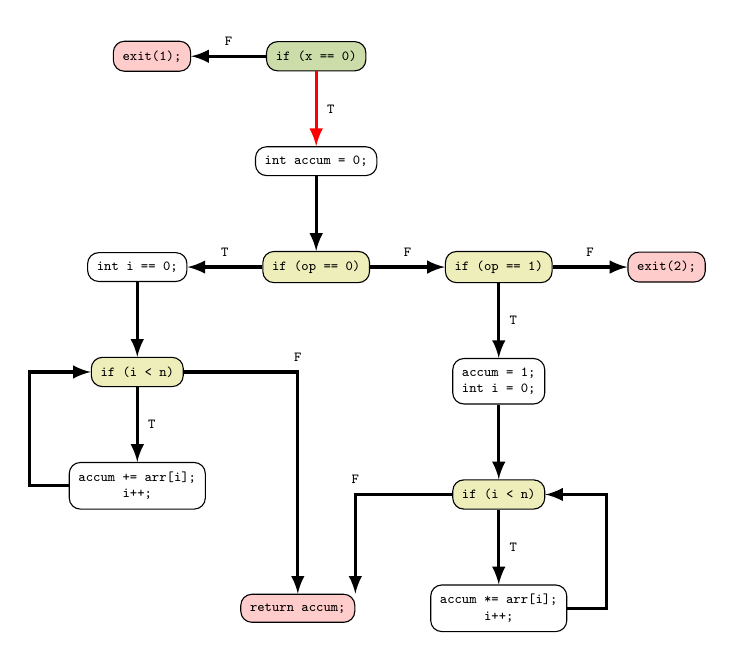
\begin{tikzpicture}[auto,
  start chain = going below,
  node distance = .95 cm,
  font=\tiny\ttfamily
]

\node[decision, fill=pale-green] (b0) {if (x == 0)};
\node[stop, left=of b0] (b1) {exit(1);};
\node[box, below=of b0] (b2) {int accum = 0;};
\node[decision, below=of b2] (b3) {if (op == 0)};
\node[box, left=of b3] (b4) {int i == 0;};
\node[decision, below=of b4] (b5) {if (i < n)};
\node[box, below=of b5] (b6) {
  accum += arr[i]; \\
  i++;
};
% b12 needs to be defined before b7
\node[decision, right=of b3] (b8) {if (op == 1)};
\node[stop, right=of b8] (b9) {exit(2);};
\node[box, below=of b8] (b10) {
  accum = 1; \\
  int i = 0;
};
\node[decision, below=of b10] (b11) {if (i < n)};
\node[box, below=of b11] (b12) {
  accum *= arr[i];\\
  i++;
};
\node[stop, below=of b3, left=of b12] (b7) {return accum;};

\draw[arr]  (b0) -- (b1) node[midway, above]{F};
\draw[arr, draw=red]  (b0) -- (b2) node[midway, right]{T};
\draw[arr]  (b2) -- (b3);
\draw[arr]  (b3) -- (b4) node[midway, above]{T};
\draw[arr]  (b3) -- (b8) node[midway, above]{F};
\draw[arr]  (b8) -- (b9) node[midway, above]{F};
\draw[arr]  (b8) -- (b10) node[midway, right]{T};
\draw[arr]  (b10) -- (b11);
\draw[arr]  (b11) -- (b12) node[midway, right]{T};
\draw[arr]  (b12.east) -- ++ (.5, 0) |- (b11);
\draw[arr]  (b11) -- ++ (-.75, 0) -| (b7.north east) node[midway, above]{F};
\draw[arr]  (b4) -- (b5);
\draw[arr]  (b5) -- (b6) node[midway, right]{T};
\draw[arr]  (b6.west) -- ++ (-.5,0) |- (b5);
\draw[arr]  (b5.east) -- ++ (.25, 0) -| (b7) node[midway, above]{F};



\end{tikzpicture}

%% \end{frame}

%% \begin{frame}
%% \frametitle{Example: finding an input to reach a desired state}
%%   \vspace{-.75cm}\centering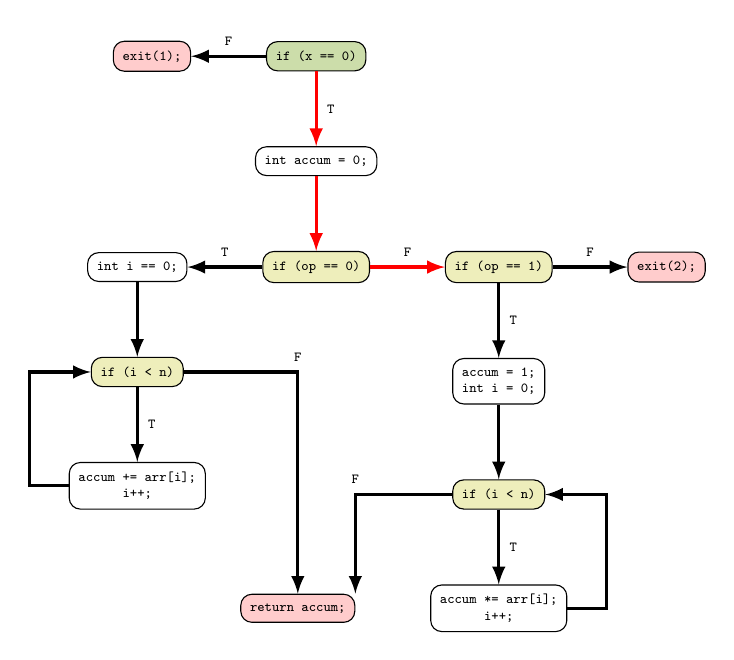
\begin{tikzpicture}[auto,
  start chain = going below,
  node distance = .95 cm,
  font=\tiny\ttfamily
]

\node[decision, fill=pale-green] (b0) {if (x == 0)};
\node[stop, left=of b0] (b1) {exit(1);};
\node[box, below=of b0] (b2) {int accum = 0;};
\node[decision, below=of b2] (b3) {if (op == 0)};
\node[box, left=of b3] (b4) {int i == 0;};
\node[decision, below=of b4] (b5) {if (i < n)};
\node[box, below=of b5] (b6) {
  accum += arr[i]; \\
  i++;
};
% b12 needs to be defined before b7
\node[decision, right=of b3] (b8) {if (op == 1)};
\node[stop, right=of b8] (b9) {exit(2);};
\node[box, below=of b8] (b10) {
  accum = 1;\\
  int i = 0;
};
\node[decision, below=of b10] (b11) {if (i < n)};
\node[box, below=of b11] (b12) {
  accum *= arr[i];\\
  i++;
};
\node[stop, below=of b3, left=of b12] (b7) {return accum;};

\draw[arr]  (b0) -- (b1) node[midway, above]{F};
\draw[arr, draw=red]  (b0) -- (b2) node[midway, right]{T};
\draw[arr, draw=red]  (b2) -- (b3);
\draw[arr]  (b3) -- (b4) node[midway, above]{T};
\draw[arr, draw=red]  (b3) -- (b8) node[midway, above]{F};
\draw[arr]  (b8) -- (b9) node[midway, above]{F};
\draw[arr]  (b8) -- (b10) node[midway, right]{T};
\draw[arr]  (b10) -- (b11);
\draw[arr]  (b11) -- (b12) node[midway, right]{T};
\draw[arr]  (b12.east) -- ++ (.5, 0) |- (b11);
\draw[arr]  (b11) -- ++ (-.75, 0) -| (b7.north east) node[midway, above]{F};
\draw[arr]  (b4) -- (b5);
\draw[arr]  (b5) -- (b6) node[midway, right]{T};
\draw[arr]  (b6.west) -- ++ (-.5,0) |- (b5);
\draw[arr]  (b5.east) -- ++ (.25, 0) -| (b7) node[midway, above]{F};



\end{tikzpicture}

%% \end{frame}

\begin{frame}
\frametitle{Example: finding an input to reach a desired state}
  \vspace{-.75cm}\centering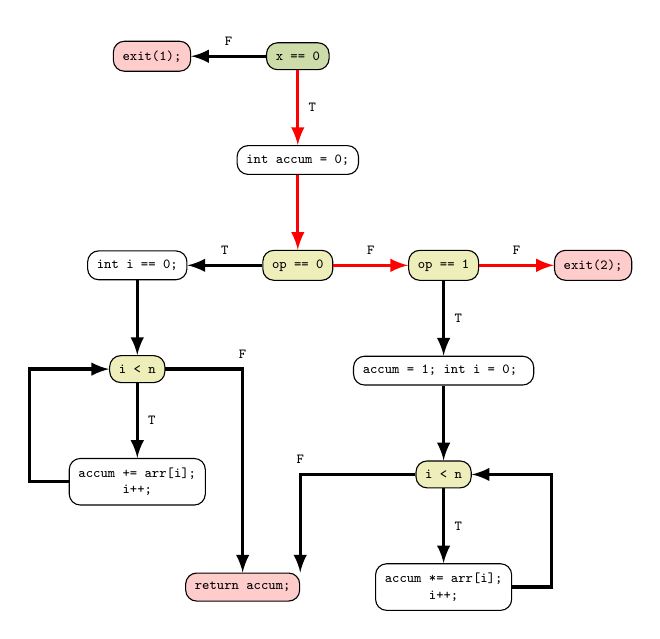
\begin{tikzpicture}[auto,
  start chain = going below,
  node distance = .95 cm,
  font=\tiny\ttfamily
]

\node[decision, fill=pale-green] (b0) {x == 0};
\node[stop, left=of b0] (b1) {exit(1);};
\node[box, below=of b0] (b2) {int accum = 0;};
\node[decision, below=of b2] (b3) {op == 0};
\node[box, left=of b3] (b4) {int i == 0;};
\node[decision, below=of b4] (b5) {i < n};
\node[box, below=of b5] (b6) {
  accum += arr[i]; \\
  i++;
};
% b12 needs to be defined before b7
\node[decision, right=of b3] (b8) {op == 1};
\node[stop, right=of b8] (b9) {exit(2);};
\node[box, below=of b8] (b10) {
  accum = 1;
  int i = 0;
};
\node[decision, below=of b10] (b11) {i < n};
\node[box, below=of b11] (b12) {
  accum *= arr[i];\\
  i++;
};
\node[stop, below=of b3, left=of b12] (b7) {return accum;};

\draw[arr]  (b0) -- (b1) node[midway, above]{F};
\draw[arr, draw=red]  (b0) -- (b2) node[midway, right]{T};
\draw[arr, draw=red]  (b2) -- (b3);
\draw[arr]  (b3) -- (b4) node[midway, above]{T};
\draw[arr, draw=red]  (b3) -- (b8) node[midway, above]{F};
\draw[arr, draw=red]  (b8) -- (b9) node[midway, above]{F};
\draw[arr]  (b8) -- (b10) node[midway, right]{T};
\draw[arr]  (b10) -- (b11);
\draw[arr]  (b11) -- (b12) node[midway, right]{T};
\draw[arr]  (b12.east) -- ++ (.5, 0) |- (b11);
\draw[arr]  (b11) -- ++ (-.75, 0) -| (b7.north east) node[midway, above]{F};
\draw[arr]  (b4) -- (b5);
\draw[arr]  (b5) -- (b6) node[midway, right]{T};
\draw[arr]  (b6.west) -- ++ (-.5,0) |- (b5);
\draw[arr]  (b5.east) -- ++ (.25, 0) -| (b7) node[midway, above]{F};



\end{tikzpicture}

% mention that targets are not always terminal nodes in practice.
% they might not even be specific nodes, but rather any node that meets a set of conditions based on the modeled execution of the program (i.e., we have to check this after every relevant step
\end{frame}


\begin{frame}
\frametitle{Why is this hard?}
\begin{itemize}
\item{Complexity}
  % path explosion; what do I do about loops?
  \medskip
\item{Undecidability}
% mention halting problem: determine for a given program and a given input, will this program terminate? Turing proved that a general algorithm for all possible program-input pairs does not exist, i.e. we cannot decide yes or no.
  \medskip
\item{Leaky abstractions}
% example: buffer overflow - unless we explicitly insert check on length in C, without special intervention (e.g., compiler pass), it won't be done in the asm. This is different to other application programming languages, and has led to many security problems
  \medskip
\item{Imprecise models}
  % might not have source code, so we have to "reverse engineer" / decompile, which is hard
  % there's actually a lower level under assembly, called the microarchitecture of the processor, which is often proprietary. Does not affect the analysis I'm showing today, but very important for low-level security properties, e.g. cryptographic constant time.
\end{itemize}
\end{frame}
  
  
\begin{frame}
  \frametitle{Interlude: mathematical logic}
  \begin{itemize}
  \item{\textbf{Formal language}: set of symbols (aka \textit{alphabet}) + rules for putting them together into sentences (aka \textit{well-formed formulae (wff))}}
    \medskip
  \item{\textbf{Theory}: a set of sentences in a formal language}
    \medskip
  \item{\textbf{Decision problem}: a yes-or-no question over a set of input values}
    % we talked about one just now - the halting problem
    % in general, classified by the computational resources required to solve
\end{itemize}
\end{frame}

\begin{frame}
  \frametitle{Interlude: mathematical logic}
  \begin{itemize}
  \item{\textbf{Propositional calculus}: propositional variables + logical connectives \\
    + inference rules + axioms}
    \medskip
  \item{\textbf{Boolean satisfiability (SAT)}: is there an assignment of variables to T/F such that the formula evaluates to T?}
    % NP-complete
  \end{itemize}
\end{frame}

\begin{frame}
  \frametitle{Example: propositional calculus}
  \begin{displaymath}
    \begin{array}{c c | c}
      P & Q & P \oplus Q\\
      \hline
      \rowcolor{pale-green} T & T & T\\
      T & F & F\\
      F & T & F\\
      F & F & F\\
      \end{array}
  \end{displaymath}
  \bigskip
  \center $(P, Q) = (T, T)$ \textbf{\textit{satisfies}} $P \oplus Q$.
  % remark - sometimes called zero'th-order logic
\end{frame}

\begin{frame}
  \frametitle{Interlude: mathematical logic}
  \begin{itemize}
  \item{\textbf{First-order logic}: variables + logical connectives 
    + inference rules + axioms \textbf{+ quantifiers ($\forall$, $\exists$) 
      + (often) equality ($=$) \\ 
      + predicates + functions} }
    \medskip
  \item{\textbf{Satisfiability modulo theories (SMT)}: is there an assignment of variables to values such that the formula evaluates to true?}
    % generalization of SAT
  \end{itemize}
\end{frame}

\begin{frame}
  \frametitle{Example: (first-order) theory of integers}
  \begin{displaymath}
    \begin{cases}
      5x + 4y - z = 0 \\
      10y - 3z = 11 \\
      z = 3
    \end{cases}
  \end{displaymath}
  
  \center\[ \exists (x, y, z \in \mathbb{Z})(
  (5x + 4y -z = 0) \wedge
  (10y - 3z = 11) \wedge
  (z = 3))
  \]
  
\center $(x, y, z) = (-1, 2, 3)$ is a \textbf{\textit{satisfying assignment}} for the above system.
\end{frame}

\begin{frame}
  \frametitle{Example: now with path constraints!}
  \begin{columns}
  \column{.7\linewidth}{
      \vspace{-.8cm}\centering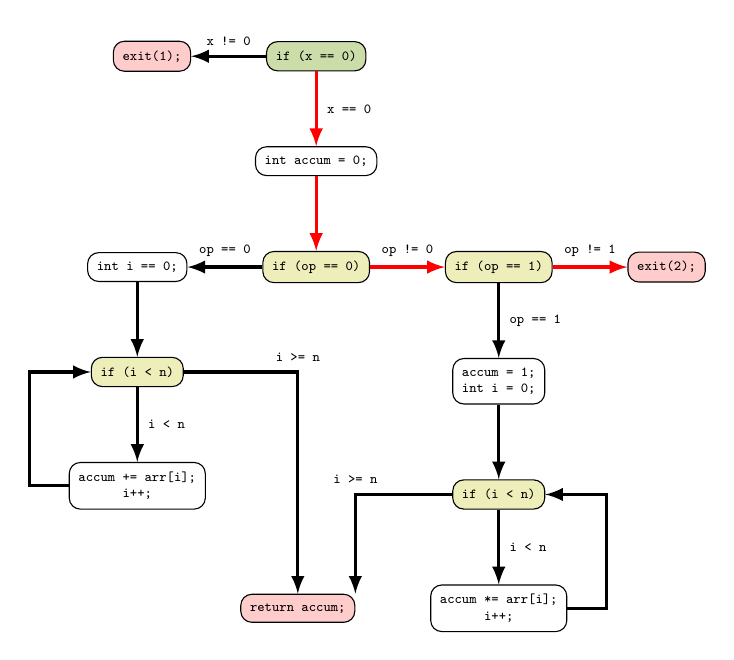
\begin{tikzpicture}[auto,
  start chain = going below,
  node distance = .95 cm,
  font=\tiny\ttfamily
]

\node[decision, fill=pale-green] (b0) {if (x == 0)};
\node[stop, left=of b0] (b1) {exit(1);};
\node[box, below=of b0] (b2) {int accum = 0;};
\node[decision, below=of b2] (b3) {if (op == 0)};
\node[box, left=of b3] (b4) {int i == 0;};
\node[decision, below=of b4] (b5) {if (i < n)};
\node[box, below=of b5] (b6) {
  accum += arr[i]; \\
  i++;
};
% b12 needs to be defined before b7
\node[decision, right=of b3] (b8) {if (op == 1)};
\node[stop, right=of b8] (b9) {exit(2);};
\node[box, below=of b8] (b10) {
  accum = 1;\\
  int i = 0;
};
\node[decision, below=of b10] (b11) {if (i < n)};
\node[box, below=of b11] (b12) {
  accum *= arr[i];\\
  i++;
};
\node[stop, below=of b3, left=of b12] (b7) {return accum;};

\draw[arr]  (b0) -- (b1) node[midway, above]{x != 0};
\draw[arr, draw=red]  (b0) -- (b2) node[midway, right]{x == 0};
\draw[arr, draw=red]  (b2) -- (b3);
\draw[arr]  (b3) -- (b4) node[midway, above]{op == 0};
\draw[arr, draw=red]  (b3) -- (b8) node[midway, above]{ op != 0};
\draw[arr, draw=red]  (b8) -- (b9) node[midway, above]{ op != 1};
\draw[arr]  (b8) -- (b10) node[midway, right]{op == 1};
\draw[arr]  (b10) -- (b11);
\draw[arr]  (b11) -- (b12) node[midway, right]{ i < n};
\draw[arr]  (b12.east) -- ++ (.5, 0) |- (b11);
\draw[arr]  (b11) -- ++ (-.75, 0) -| (b7.north east) node[midway, above]{ i >= n};
\draw[arr]  (b4) -- (b5);
\draw[arr]  (b5) -- (b6) node[midway, right]{ i < n};
\draw[arr]  (b6.west) -- ++ (-.5,0) |- (b5);
\draw[arr]  (b5.east) -- ++ (.25, 0) -| (b7) node[midway, above]{i >= n};



\end{tikzpicture}

    }
  \column{.3\linewidth}{
    \small{
      Is the ``\texttt{exit(2);}'' node reachable?
      
      \bigskip
      \bigskip
      \bigskip
$\exists ((x, op, n \in int)$\\
$(arr \in List[int]))($\\
$(x != 0) \mbox{ \&\&} $ \\
$(op != 0) \mbox{ \&\&} $ \\
$(op != 1))$

\medskip
Satisfying assignments: $(x \in int \setminus \{0\}) \mbox{ \&\&} $ \\
($op \in int \setminus \{0, 1\})$; \\
$arr$, $n$ unconstrained
  }}
\end{columns}
  
\end{frame}

 \begin{frame}
\frametitle{Can we automate program analysis tasks?}
\begin{itemize}
\item{Yes! (But we might have to make some simplifications to make problems tractable, compromising soundness and/or completeness.)}
  % soundness prevents false negatives, i.e., all possible unsafe inputs are guaranteed to be found
  % completeness prevents false positives, i.e., input values deemed unsafe are actually unsafe
  \medskip
  \item{One way: build analysis systems using SMT solvers.}
    \medskip
  \item{Example theories: integers, bit-vectors, arrays}
      \end{itemize}
  \end{frame}

%%   \begin{frame}
%% \frametitle{Example: using angr to find our path}
  
%%   \end{frame}

\begin{frame}
\frametitle{Where can mathematicians help?}
\begin{itemize}
\item{Modeling}
  \medskip
\item{Search strategies}
  \medskip
\item{Incorporating information from other analyses}
  \end{itemize}
\end{frame}

% what's the goal at the end of the day?
% find vulnerabilities (preferably exploitable ones that lead to arbitrary code execution)
% fix your code, and develop generalized mitigations if possible

\appendix

\begin{frame}
\frametitle{Graphs in computer network defense}
Example: network intrusion detection
\bigskip
\begin{itemize}
  \item{Nodes - computers on a network (aka ``hosts''), labeled by IP addresses}
    \medskip
  \item{Edges - communication between hosts}
  \end{itemize}
  \end{frame}

   \begin{frame}
\frametitle{Graphs in computer network defense}
Example: Internet topology analysis
\bigskip
\begin{itemize}
  \item{Nodes - routers that advertise eBGP routes}
    \medskip
  \item{Edges - advertised connectivity between ``peered'' routers}
  \end{itemize}
  \end{frame}




\end{document}
